\documentclass[12pt,a4paper]{article}
\usepackage[catalan]{babel}
\usepackage[utf8]{inputenc}

\usepackage[right=1cm,left=1.5cm,top=4cm,bottom=2cm,headsep=0.5cm, footskip=0.5cm]{geometry}
\usepackage{graphicx,subfigure}
\usepackage{amsmath,amssymb}
\usepackage{underscore}
\usepackage{fancyhdr}
\usepackage{array}
\usepackage{yhmath}

\graphicspath{ {img/} }

\pagestyle{fancy}
\fancyhf{}
\rhead{\textbf{Alberto Navalón Lillo}}
\lhead{\textit{Geometria: teoremes, conceptes i figures}}

\begin{document}

\section{Teorema de Pitàgores}

Per a fer servir el teorema de Pitàgores necessitem un triangle rectangle (figura A). A un triangle rectangle, com a tots els triangles, hi ha tres costats, però als rectangles, el més llarg de tots s'anomena \textit{hipotenusa}, mentre que els altres dos, una mica més curts, són \textit{catets} i, el més important és que als triangles rectangles \textbf{un dels angles sempre és recte}, és a dir, de 90º.\\

\begin{figure}[h]
	\centering
	\subfigure[Fig. A: representació d'un triangle rectangle.]{
		\label{fig:a}
		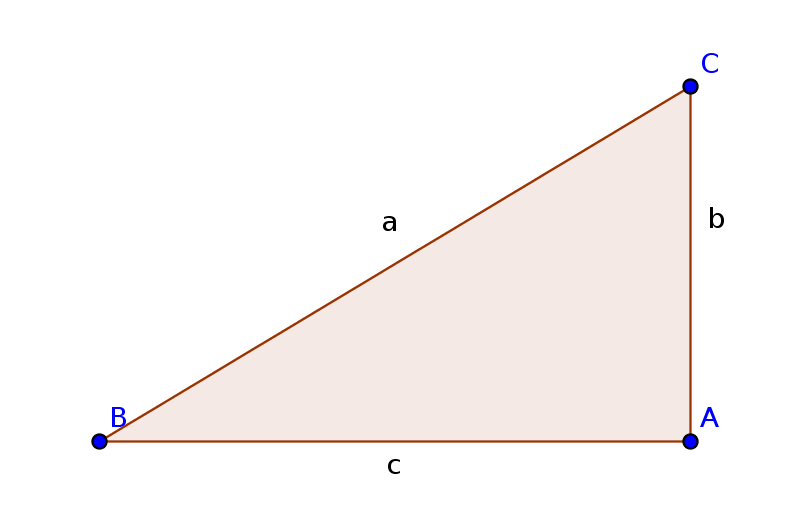
\includegraphics[width=6cm]{trianglerectangle}
	}
\end{figure}

Ara, per al triangle presentat en la figura, necessitem almenys la longitud de dos dels costats per a poder trobar el restant. Per això donarem valor als dos catets, \(b=3cm \text{ i } c=4cm\). Una vegada tenim aquests valors, podem continuar a calcular la llargària del costat que ens queda, el qual és, en aquest cas, la hipotenusa (\textit{a}). Plantegem l'equació i resolem:

\[
	a^2=b^2+c^2 \Rightarrow a^2=3^2+4^2=25 \Rightarrow a=\sqrt{25}=5cm
\]

\section{Teorema de Tales}

L'anomenat \textit{teorema de Tales} s'enuncia com:\\

\indent\textit{Si dues rectes }r\textit{, }s\textit{ són tallades per rectes paral·leles }a\textit{, }b\textit{, }c\textit{, els segments que es formen conseqüentment son proporcionals.}\\

Podem observar una representació d'una aplicació del teorema a la imatge següent:

\begin{figure}[h]
	\centering
	\subfigure[Fig. B: representació del teorema de Tales.]{
		\label{fig:b}
		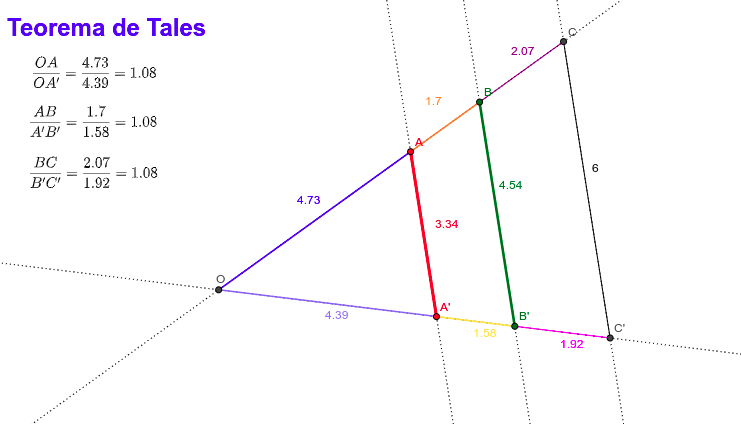
\includegraphics[width=8.5cm]{teorematales}
	}
\end{figure}

\section{Simetria}

La simetria és la correspondència exacta en forma, tamany i posició de les parts d'alguna cosa. Hi ha diferents tipus de simetries. Les més importants i representatives són la \textbf{simetria bilateral}, la \textbf{simetria radial} i la \textbf{asimetria} (falta de qualsevol tipus de simetria), i estos tres es troben fundamentalment en la biologia. També podem trobar altres exemples de simetria, els quals són més comuns a matemàtiques:

\begin{itemize}
	\item Simetria \textbf{axial} (equivalent a la simetria bilateral): fundamentalment, aquesta és la simetria que es dóna al voltant d'un eix. A la figura C podem observar un exemple representat d'aquest tipus de simetria.
	\item Simetria \textbf{especular} (similar al funcionament d'un espill): ací, l'eix de simetria no talla en cap moment a la figura.
	\item Simetria \textbf{esfèrica}.
	\item Simetria \textbf{translacional}.
	\item Simetria \textbf{helicoidal}.
	\item Simetria de \textbf{rotoreflexió}.
\end{itemize}

\begin{figure}[h]
	\centering
	\subfigure[Fig. C: representació de la simetria axial.]{
		\label{fig:c}
		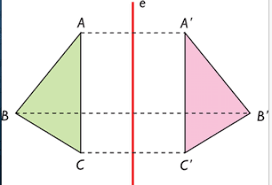
\includegraphics[width=6.5cm]{simetriaaxial}
	}
\end{figure}

\section{Poliedres}

Els \textbf{poliedres} són, en poques paraules, figures tridimensionals limitades per polígons, els quals són les cares d'aquest poliedre. Per a donar nom a aquests poliedres, utilitzem els prefixos grecs \textit{tetra-}, \textit{penta-}, \textit{hexa-}, \textit{hepta-}... i l'ajuntem amb \textit{-edre}, de forma que aconseguim noms com \textit{tetraedre} (poliedre de quatre cares), \textit{pentaedre} (cinc cares), \textit{hexaedre} (sis cares), \textit{heptaedre} (set cares), \textit{octoedre} (huit cares), \textit{decaedre} (deu cares), o \textit{dodecaedre} (dotze cares).\\

També és important mencionar que els poliedres es formen a partir de tres elements fundamentals: les \textbf{cares}, les \textbf{aristes} i els \textbf{vèrtexs}. Per a mesurar els poliedres, podem calcular el seu \textbf{volum}, o l'\textbf{àrea total} de la seua superfície, que és la suma de les àrees de totes les cares.

\subsection{Àrees i volums de poliedres}

Per sort o per desgràcia, la majoria dels poliedres requereixen una fórmula diferent per a calcular ja siga l'àrea total o el volum. Per tant, ací són les fórmules per als poliedres més importants:

\begin{itemize}
	\item \textbf{Cub/Hexaedre}\footnote{La variable \textit{a} representa la llargària d'una de les aristes, ja que són totes iguals.}: \(A_T=6a^2 \mid V=a^3\)
	\item \textbf{Paral·lelepípede/Ortoedre}\footnote{Un paral·lelepípede o ortoedre és un poliedre de sis cares rectangulars, no quadrades (cub).} \footnote{Les variables \textit{a}, \textit{b} i \textit{c} representen l'altura, l'amplària i la profunditat de l'ortoedre, respectivament}: \(A=2(ab+ac+bc) \mid V=abc\)
	\item \textbf{Prisma}: \(A_T=2A_B+A_L \mid V=A_B \cdot h\)
	\item \textbf{Cilindre}: \(A_T=2A_B+A_L \Rightarrow A_T=2(\pi r^2)+2\pi rh \mid V=A_B \cdot h \Rightarrow V=\pi r^2h\)
	\item \textbf{Piràmide}: \(A_T=A_B+A_L \mid V=\frac{1}{3}A_B \cdot h\)
	\item \textbf{Con}\footnote{La variable \textit{g} representa la generatriu del con.}: \(A_T=A_B+A_L \Rightarrow A_T=\pi r^2+\pi rg \mid V=\frac{1}{3}A_B \cdot h \Rightarrow V=\frac{1}{3}\pi r^2\sqrt{g^2-r^2}\)
	\item \textbf{Tronc de piràmide}: \(A_T=A_{B_M}+A_{B_m}+A_L \mid V=\frac{1}{3}(A_{B_M}+A_{B_m}+ \sqrt{A_{B_M} \cdot A_{B_m}}) \cdot h\)
	\item \textbf{Tronc de con}: \(A_T=A_{B_M}+A_{B_m}+A_L \Rightarrow A_T=\pi R^2+\pi r^2+\pi(R+r)g \mid V=\frac{1}{3}(A_{B_M}+A_{B_m}+\sqrt{A_{B_M} \cdot A_{B_m}}) \cdot h \Rightarrow V=\frac{1}{3}(\pi R^2+\pi r^2+\sqrt{2\pi(R \cdot r)^2}) \cdot \sqrt{g^2-(R-r)^2}\)
	\item \textbf{Esfera}: \(A_T=4\pi r^2 \mid V=\frac{4}{3}\pi r^3\)
\end{itemize}

\end{document}